\subsection{Benefits of Top-Loading Your Short HF Vertical Antenna!}

\begin{tcolorbox}[colback=gray!10, colframe=black, title=E9D07] What is an advantage of top loading an electrically short HF vertical antenna?
\begin{enumerate}[label=\Alph*.]
    \item Lower Q
    \item Greater structural strength
    \item Higher losses
    \item \textbf{Improved radiation efficiency}
\end{enumerate} \end{tcolorbox}

\subsubsection{Understanding Vertical Antennas}
An electrically short vertical antenna is one that is significantly shorter than a quarter wavelength of the frequency it is intended to transmit or receive. Due to its short height, this type of antenna typically suffers from high losses and reduced radiation efficiency. 

Top loading is a technique used to improve the performance of short vertical antennas. By adding horizontal elements or conductors at the top of the antenna, the overall effective height is increased, which can enhance its radiation efficiency. 

\subsubsection{Related Concepts}
To understand the advantage of top-loading an electrically short HF vertical antenna, one must consider several key concepts:

\begin{itemize}
    \item \textbf{Radiation Efficiency}: This is the measure of how effectively the antenna radiates radio frequency (RF) energy compared to the energy lost due to resistance in the antenna.
    \item \textbf{Q Factor}: The quality factor (Q) of an antenna describes its bandwidth relative to its center frequency. A lower Q indicates a wider bandwidth.
    \item \textbf{Impedance Matching}: The mismatch between the antenna's feed point impedance and the transmission line can lead to reflections and losses.
\end{itemize}

\subsubsection{Calculating Radiation Efficiency}
The radiation efficiency (\(\eta\)) of an antenna can be calculated using the formula:

\[
\eta = \frac{R_r}{R_r + R_l}
\]

where:
- \(R_r\) is the radiation resistance (typically less for short antennas)
- \(R_l\) is the loss resistance (due to ohmic losses)

In a short vertical antenna, both \(R_r\) and \(R_l\) can vary significantly based on design and loading techniques. By top loading, \(R_r\) can be effectively increased while minimizing \(R_l\), thereby improving \(\eta\).

\subsubsection{Diagram}
If necessary, the antenna configuration for a top-loaded vertical antenna can be visualized as follows:

\begin{center}
\usetikzlibrary{shapes, arrows}
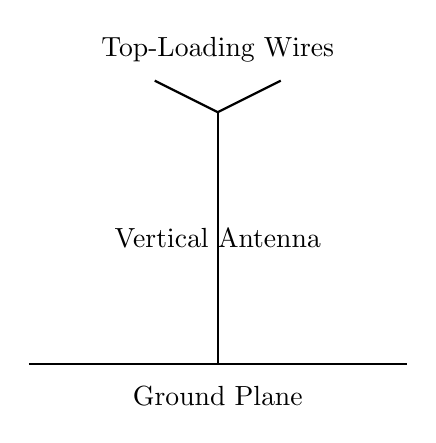
\begin{tikzpicture}[scale=0.8]
    % Draw antenna pole
    \draw[thick] (0,0) -- (0,4);
    % Draw top loading elements
    \draw[thick] (0,4) -- (-1,4.5);
    \draw[thick] (0,4) -- (1,4.5);
    % Draw ground plane
    \draw[thick] (-3,0) -- (3,0);
    % Add labels
    \node at (0, 5) {Top-Loading Wires};
    \node at (0, -0.5) {Ground Plane};
    \node at (0, 2) {Vertical Antenna};
\end{tikzpicture}
\end{center}

In conclusion, top loading an electrically short HF vertical antenna significantly improves its radiation efficiency, offering a clear operational benefit. This technique is particularly valuable for operators who wish to enhance the performance of their compact antenna designs.
